\subsection{支持向量机}
\label{sec:classification-svm}

感知机回答了一个基本问题：如果训练样本能够被某个超平面分开，怎样通过错误驱动的更新找到一个分离器？但分开训练样本并不意味着分界的位置已经合适。同一批可分数据往往允许许多分离超平面，即使从零参数开始，感知机的结果仍会受样本顺序和更新规则影响。一个紧贴训练样本的边界虽然没有训练错误，却可能在输入受到很小扰动时改变预测。要在这些分离器之间作出选择，还需要说明什么样的边界更值得保留。

\term{支持向量机}（support vector machine，SVM）以训练样本到边界的距离选择分隔面：在正确分离样本的前提下，增大最近样本到边界的距离，称为最大间隔。给定特征表示与距离度量后，这个几何准则使边界具有可比较的尺度。不可分数据可以通过松弛约束处理，非线性关系则可以通过改变特征表示处理；两种扩展分别作用于误差容忍与候选函数。Boser、Guyon与Vapnik在1992年把最大间隔训练与核表示结合，Cortes与Vapnik在1995年进一步系统发展了容许间隔违反的形式，前者改变非线性特征的使用方式，后者让噪声或类别重叠进入带惩罚的训练目标\scite{boser1992margin,cortes1995}。下面先从可分数据推导间隔目标与对偶，再用SMO说明参数怎样求出，然后分别改变误差容忍、输入表示与间隔调节。

\subsubsection{模型结构}
\label{sec:classification-svm-model}

\paragraph{得分与类别规则}
沿用二分类标签约定，设训练集为$D_n=\{(\bm{x}_i,y_i)\}_{i=1}^n$，其中$\bm{x}_i\in\mathbb{R}^d$、$y_i\in\{-1,+1\}$，并假设两类均非空。令实值得分为$g(\bm{x})=\bm{w}^{\top}\bm{x}+b$，其中$\bm{w}\in\mathbb{R}^d$、$b\in\mathbb{R}$且$\bm{w}\ne\bm{0}$。决策超平面是$g(\bm{x})=0$，预测规则为$\hat y(\bm{x})=\operatorname{sign}(g(\bm{x}))$；若得分恰为零，约定预测为$+1$。

\paragraph{函数间隔与几何间隔}
仅比较$y_i g(\bm{x}_i)$还不能比较不同超平面。把$(\bm{w},b)$同时乘以任意正数，分类结果不变，这个数值却会随之放大：同一条直线，把权重都乘以$100$，每个样本的得分也乘以$100$，直线却毫无变化。因此得分本身的“大小”带有任意性，不能直接当作距离或安全裕度。为区分参数尺度与真实距离，定义样本的\term{函数间隔}（functional margin）为$m_i=y_i g(\bm{x}_i)$，定义其\term{几何间隔}（geometric margin）为
\begin{equation}
  \gamma_i
  =\frac{y_i(\bm{w}^{\top}\bm{x}_i+b)}
         {\lVert\bm{w}\rVert_2},
  \qquad
  \gamma=\min_{1\le i\le n}\gamma_i.
  \label{eq:classification-svm-margin}
\end{equation}
函数间隔保留了得分的尺度；几何间隔除以法向量长度，得到沿法向方向测量的有符号距离。乘上真实标签后的得分满足$y_i g(\bm x_i)>0$时，样本位于正确类别一侧，这个距离为正。$g(\bm x_i)=0$时，样本就在决策边界上：正类虽然按平局规则被判对，几何间隔仍为零，因而没有正半径的扰动容忍保证。

\subsubsection{参数学习}
\label{sec:classification-svm-learning}

\paragraph{硬间隔目标与对偶参数}
严格线性可分意味着存在$(\bm{w},b)$使所有$m_i>0$。由于样本数有限，可以将这组参数除以$\min_i m_i$，得到$\min_i m_i=1$的规范化表示。在该表示下，最近样本到决策超平面的单侧距离为$1/\lVert\bm{w}\rVert_2$；两个平行超平面$g(\bm{x})=+1$与$g(\bm{x})=-1$之间的总宽度则是$2/\lVert\bm{w}\rVert_2$。本节将前者记为$\gamma$，不把单侧间隔与两侧带宽混用。

最大化$\gamma$于是等价于最小化$\lVert\bm{w}\rVert_2$。平方与正比例因子不改变最优解，却使求导更方便，得到\term{硬间隔}（hard margin）SVM的原始问题：
\begin{equation}
  \begin{aligned}
    \min_{\bm{w},b}\quad&
      \frac12\lVert\bm{w}\rVert_2^2\\
    \text{s.t.}\quad&
      y_i(\bm{w}^{\top}\bm{x}_i+b)\ge1,
      \quad i=1,\ldots,n.
  \end{aligned}
  \label{eq:classification-svm-hard-primal}
\end{equation}
这里的“硬”表示每个样本都必须满足间隔约束，不能用其他样本的改善来补偿某个样本的违反。约束写为大于等于$1$并没有放弃规范化：若一个可行解的最小函数间隔严格大于$1$，将参数一起缩小就能降低目标，所以最优解必有紧约束。

\begin{example}[单侧间隔与带宽]
  \label{ex:classification-svm-one-dimensional}
  考虑一维教学数据$(x_1,y_1)=(-1,-1)$、$(x_2,y_2)=(1,+1)$、$(x_3,y_3)=(-2,-1)$和$(x_4,y_4)=(2,+1)$。任意落在$-1$与$1$之间的阈值都能正确分类，但只有阈值$0$使两侧最近距离的较小者达到最大。规范化最优解为$w^{\ast}=1$、$b^{\ast}=0$；最近样本的单侧距离为$1$，两条支持超平面在此退化为两个点$-1$与$1$，其间距离为$2$。更远的两个样本不限制这一最优间隔。
\end{example}

每个间隔约束对最优边界的影响，可由对应的拉格朗日乘子表示。原问题是在“选一条直线”，让它离样本尽量远；对偶则换一个视角，改问“每个训练样本对这条直线有多大约束力”。每个样本分到一个非负权重$\alpha_i$，离边界远、不构成约束的样本权重为零，真正“撑住”边界两侧的少数样本权重为正，它们就是后面的支持向量。\term{对偶问题}（dual problem）把这些约束权重作为优化变量，既揭示参与预测的样本，也把训练表示为样本间内积运算，为核化提供入口。原始与对偶的变量数分别受特征维数和样本数影响，计算选择还要结合求解器与数据稀疏性。

将约束写为$1-y_i(\bm{w}^{\top}\bm{x}_i+b)\le0$，引入$\alpha_i\ge0$，记$\bm{\alpha}=(\alpha_1,\ldots,\alpha_n)^{\top}$。拉格朗日函数为
\begin{equation}
  \begin{aligned}
    L(\bm{w},b,\bm{\alpha})
    ={}&\frac12\lVert\bm{w}\rVert_2^2\\
      &+\sum_{i=1}^n\alpha_i
        \bigl[1-y_i(\bm{w}^{\top}\bm{x}_i+b)\bigr].
  \end{aligned}
  \label{eq:classification-svm-hard-lagrangian}
\end{equation}
这是一个凸二次规划：在严格可分条件下存在严格满足不等式的可行点，故强对偶成立，即对拉格朗日函数先消去$(\bm{w},b)$、再对乘子最大化与原问题同解。下面据此计算对偶目标。

现在计算$q(\bm{\alpha})=\inf_{\bm{w},b}L(\bm{w},b,\bm{\alpha})$。由于$b$没有二次项，若$\sum_i\alpha_i y_i\ne0$，沿$b$的某个方向就有$L\to-\infty$。要使$q$有限，必须满足等式约束；关于$\bm{w}$的极小值则由驻点给出：
\begin{equation}
  \bm{w}=\sum_{i=1}^n\alpha_i y_i\bm{x}_i,
  \qquad
  \sum_{i=1}^n\alpha_i y_i=0.
  \label{eq:classification-svm-stationarity}
\end{equation}
令$\bm{v}=\sum_i\alpha_i y_i\bm{x}_i$，代入后涉及权重的两项变为$\frac12\lVert\bm{v}\rVert_2^2-\lVert\bm{v}\rVert_2^2$，而$b$项为零。展开$\lVert\bm{v}\rVert_2^2$，便得到
\begin{equation}
  \begin{aligned}
    \max_{\bm{\alpha}}\quad&
      q(\bm{\alpha})
      =\sum_{i=1}^n\alpha_i
       -\frac12\sum_{i,j=1}^n
          \alpha_i\alpha_j y_i y_j
          \bm{x}_i^{\top}\bm{x}_j\\
    \text{s.t.}\quad&
      \sum_{i=1}^n\alpha_i y_i=0,\qquad
      \alpha_i\ge0,\quad i=1,\ldots,n.
  \end{aligned}
  \label{eq:classification-svm-hard-dual}
\end{equation}
二次项矩阵的元素为$\bm{Q}_{i,j}=y_i y_j\bm{x}_i^{\top}\bm{x}_j$。对任意$\bm{a}\in\mathbb{R}^n$，有$\bm{a}^{\top}\bm{Q}\bm{a}=\lVert\sum_i a_i y_i\bm{x}_i\rVert_2^2\ge0$，所以$q$是凹函数；它未必严格凹，因而对偶乘子未必唯一。

原始解与对偶解的联系可以用\term{Karush--Kuhn--Tucker条件}（Karush--Kuhn--Tucker conditions，KKT条件）完整表达。它们同时检查解是否满足约束、是否达到驻点，以及一个约束是否真的限制了目标的继续改善。在当前凸问题与强对偶下，这组条件对最优性既必要又充分：
\begin{equation}
  \begin{aligned}
    &m_i^{\ast}=y_i g^{\ast}(\bm{x}_i)\ge1,
      \qquad \alpha_i^{\ast}\ge0,\\
    &\alpha_i^{\ast}(m_i^{\ast}-1)=0,
      \qquad i=1,\ldots,n,\\
    &\bm{w}^{\ast}
      =\sum_{i=1}^n\alpha_i^{\ast}y_i\bm{x}_i,
      \qquad \sum_{i=1}^n\alpha_i^{\ast}y_i=0.
  \end{aligned}
  \label{eq:classification-svm-hard-kkt}
\end{equation}
其中第三个关系是\term{互补松弛}（complementary slackness）：乘子与约束的剩余量不能同时为正。最后一行是关于权重与偏置的驻点条件。

把$\alpha_i^{\ast}>0$的样本称为\term{支持向量}（support vector），并记其索引集为$S=\{i:\alpha_i^{\ast}>0\}$。互补松弛说明，支持向量一定满足$m_i^{\ast}=1$，而$m_i^{\ast}>1$必有$\alpha_i^{\ast}=0$。反向推断却不成立：落在边界上的样本也可能具有零乘子。例如把示例\ref{ex:classification-svm-one-dimensional}中的$x_2=1$重复一次，正类边界点的乘子总和仍可为$1/2$，但这个总量可以全部分配给其中一个副本。超平面没有改变，对偶表示与支持向量索引集却可能改变。

求得$\bm{\alpha}^{\ast}$后，恢复模型只需
\begin{equation}
  \begin{aligned}
    \bm{w}^{\ast}
      &=\sum_{i\in S}\alpha_i^{\ast}y_i\bm{x}_i,\\
    b^{\ast}
      &=y_k-(\bm{w}^{\ast})^{\top}\bm{x}_k,
        \qquad k\in S.
  \end{aligned}
  \label{eq:classification-svm-recover}
\end{equation}
精确最优解下，任意支持向量都会给出同一偏置；数值计算中可以平均多个合适样本给出的估计。只有非零乘子进入预测，这就是SVM的稀疏表示。表示的实际大小取决于支持向量数，某些训练集的大部分乃至全部样本都可能具有非零乘子。

\paragraph{二元工作集更新与停止}
\label{sec:classification-svm-smo}

对偶把未知量换成了$n$个乘子，也带来了新的计算负担。整个硬/软间隔目标通过对偶与SMO在乘子上求解，并不对原始参数$(\bm w,b)$直接做梯度下降。若存储完整内积矩阵，需要$O(n^2)$空间；通用稠密求解中的一次矩阵分解就可能需要$O(n^3)$运算，具体总成本还取决于求解器与迭代次数。为了避开每轮求解大规模二次规划（目标函数为二次、约束为线性的优化问题），Platt提出了\term{序列最小优化}（sequential minimal optimization，SMO）：每次只优化一个最小的可动变量组，把整个问题分解为可解析处理的二维子问题\scite{platt1998smo}。

一次至少需要调整两个乘子，因为$\sum_i\alpha_i y_i=0$且$y_i\ne0$，单独改变一个$\alpha_i$会破坏等式约束。选择两个不同索引$i,j$，固定其余乘子，记更新前数值为$\alpha_i^{(t)},\alpha_j^{(t)}$，并令$s=y_i y_j\in\{-1,+1\}$。如果把新的$\alpha_j$写为$u$，等式约束要求
\begin{equation}
  \alpha_i(u)
  =\alpha_i^{(t)}
    +s\bigl(\alpha_j^{(t)}-u\bigr).
  \label{eq:classification-svm-smo-coupling}
\end{equation}
这样二维问题实际上只剩一个自由变量。对硬间隔，要求$u\ge0$且$\alpha_i(u)\ge0$，可行区间$[L,H]$为
\begin{equation}
  \begin{aligned}
    s=+1:\quad&
      L=0,\qquad H=\alpha_i^{(t)}+\alpha_j^{(t)},\\
    s=-1:\quad&
      L=\max\{0,\alpha_j^{(t)}-\alpha_i^{(t)}\},
      \qquad H=+\infty.
  \end{aligned}
  \label{eq:classification-svm-smo-hard-interval}
\end{equation}
同号时两乘子之和固定，因而有有限上界；异号时差固定，二者可以同时增大。这两种区间的差别来自标签符号对等式约束的影响。

为求沿这个区间的最优点，定义$\bm{K}_{i,j}=\bm{x}_i^{\top}\bm{x}_j$，并使用当前实值得分计算误差缓存
\[
  E_k=g^{(t)}(\bm{x}_k)-y_k,\qquad
  g^{(t)}(\bm{x})
  =\sum_{\ell=1}^n\alpha_\ell^{(t)}
     y_\ell\bm{x}_\ell^{\top}\bm{x}+b^{(t)}.
\]
$E_k$保留实值得分相对于标签的偏差，因而包含更新所需的距离信息；经过$\operatorname{sign}$得到的离散预测标签不再包含这部分信息。令$\Delta=u-\alpha_j^{(t)}$。由于$\Delta\alpha_i=-s\Delta$，权重变化为$y_j\Delta(\bm{x}_j-\bm{x}_i)$，代入$q$可以逐项得到
\begin{equation}
  \begin{aligned}
    q(u)-q(\alpha_j^{(t)})
      &=y_j(E_i-E_j)\Delta-\frac12\eta\Delta^2,\\
    \eta
      &=\bm{K}_{i,i}+\bm{K}_{j,j}-2\bm{K}_{i,j}\\
      &=\lVert\bm{x}_i-\bm{x}_j\rVert_2^2\ge0.
  \end{aligned}
  \label{eq:classification-svm-smo-gain}
\end{equation}
这里$q(u)$表示其余乘子固定、$\alpha_i$按式\eqref{eq:classification-svm-smo-coupling}联动后的目标。偏置不出现在对偶目标中；误差差$E_i-E_j$中的$b^{(t)}$也恰好相消。

当$\eta>0$时，一元凹二次函数的无约束最优点与区间最优点分别为
\begin{equation}
  \begin{aligned}
    u_{\mathrm{unc}}
      &=\alpha_j^{(t)}+\frac{y_j(E_i-E_j)}{\eta},\\
    \alpha_j^{(t+1)}
      &=\min\{H,\max\{L,u_{\mathrm{unc}}\}\},\\
    \alpha_i^{(t+1)}
      &=\alpha_i^{(t)}
        +s\bigl(\alpha_j^{(t)}-\alpha_j^{(t+1)}\bigr).
  \end{aligned}
  \label{eq:classification-svm-smo-update}
\end{equation}
剪裁只对一个自由变量进行，再由等式回代另一个；独立剪裁两个乘子会破坏耦合约束。若$L=H$，该变量对没有可行移动，应另选工作集。

$\eta=0$时，式\eqref{eq:classification-svm-smo-gain}变为线性函数，在有限区间上比较两个端点的目标即可；若目标恒定，保留旧值避免无效移动。严格可分的线性硬间隔问题中，$\eta=0$意味着两输入重合，它们不可能异号；同号重复点的目标沿可行线恒定。若出现零曲率、无穷上界且目标沿该方向无限增加，则应检查可分性假设、核矩阵与数值误差，并停止该次更新。

乘子更新以后还要调整偏置。记$\Delta\alpha_i=\alpha_i^{(t+1)}-\alpha_i^{(t)}$，$\Delta\alpha_j$同理。分别要求更新后的第$i$或第$j$个样本具有函数间隔$1$，解得
\begin{equation}
  \begin{aligned}
    b_i={}&b^{(t)}-E_i
       -y_i\Delta\alpha_i\bm{K}_{i,i}
       -y_j\Delta\alpha_j\bm{K}_{i,j},\\
    b_j={}&b^{(t)}-E_j
       -y_i\Delta\alpha_i\bm{K}_{i,j}
       -y_j\Delta\alpha_j\bm{K}_{j,j}.
  \end{aligned}
  \label{eq:classification-svm-smo-bias}
\end{equation}
硬间隔中，若更新后的$\alpha_i>0$，使用$b_i$；否则若$\alpha_j>0$，使用$b_j$。二者都为正且子问题精确求解时，这两个值一致；若都不能用于确定偏置，可暂取$(b_i+b_j)/2$。这一步利用当前工作集的条件更新偏置，其他样本是否满足KKT仍由后续全局扫描检查。

令$\Delta b=b^{(t+1)}-b^{(t)}$，其他样本的缓存可由
\[
  E_k^{(t+1)}
  =E_k^{(t)}
   +y_i\Delta\alpha_i\bm{K}_{i,k}
   +y_j\Delta\alpha_j\bm{K}_{j,k}
   +\Delta b
\]
更新，不必重新计算整个预测和。在示例\ref{ex:classification-svm-one-dimensional}中，从$\bm{\alpha}^{(0)}=\bm{0}$、$b^{(0)}=0$开始，选择$x_1=-1$与$x_2=1$，有$E_1=1$、$E_2=-1$、$\eta=4$，于是得到$\alpha_1=\alpha_2=1/2$和$b=0$。此时$w=1$，其余两个样本已经在间隔外；这一教学例子的最优解恰好由一次工作集更新达到；一般训练的迭代次数由后续选点与KKT误差决定。

\begin{algorithm}[硬间隔SMO的训练框架]
  \label{alg:classification-svm-smo}
  \begin{algorithmic}[1]
    \Require 两类非空且严格可分的$D_n$，容差$\varepsilon_{\mathrm{opt}}>0$，迭代上限$t_{\max}$
    \Ensure 可行乘子、偏置及停止状态
    \State 初始化$\bm{\alpha}^{(0)}=\bm{0}$、$b^{(0)}=0$、$E_k=-y_k$
    \For{$t=0,\ldots,t_{\max}-1$}
      \State 扫描KKT残差；若全部低于容差，返回“容差满足”
      \State 选取违反KKT的索引$i$，再选有可行改进的$j$
      \State 按式\eqref{eq:classification-svm-smo-hard-interval}计算$L,H$
      \State 求解一元子问题；退化时比较端点或更换变量对
      \State 联动更新两个乘子，更新$b$与误差缓存
    \EndFor
    \State 返回当前参数及“达到迭代上限，尚未认证收敛”
  \end{algorithmic}
\end{algorithm}

对于硬间隔，$\alpha_i=0$时应检查$m_i\ge1$，$\alpha_i>0$时应检查$m_i=1$，实际实现还要给“零乘子”设置数值容差。第二个变量可以优先选择误差差较大或预测目标增益较大的样本，并通过回退扫描持续检查其余违反条件的变量。算法\ref{alg:classification-svm-smo}给出共同框架，具体选点规则仍须保证持续处理违反KKT的变量。SMO避免每轮分解整个稠密二次规划矩阵，但核缓存与工作集扫描仍有成本。在线性问题中，也可以直接维护$\bm{w}$，不必先存储全部样本内积；LIBLINEAR面向大规模稀疏线性分类提供了专门求解路线\scite{fan2008liblinear}。

\subsubsection{理论分析}
\label{sec:classification-svm-analysis}

\paragraph{表达边界与局部扰动}
原坐标中的线性SVM仍只给出单个仿射半空间。增加间隔只是在同一族分离器中选择位置，并不新增异或所需的交互特征。由Cauchy--Schwarz不等式，若输入改变为$\bm{x}_i+\bm{\Delta}$，有
\[
  y_i g(\bm{x}_i+\bm{\Delta})
  \ge y_i g(\bm{x}_i)
      -\lVert\bm{w}\rVert_2\lVert\bm{\Delta}\rVert_2.
\]
因此，$\lVert\bm{\Delta}\rVert_2<\gamma_i$时预测不会翻转。这说明间隔量化当前特征空间中、由该范数限定的输入扰动容忍程度；它以给定表示和范数为条件，分布变化需要另外规定变化方式。

\paragraph{全局最优与求解条件}
有限样本严格可分且两类非空时，规范化硬间隔最优参数的存在唯一性依据如下。目标$\tfrac12\lVert\bm{w}\rVert_2^2$凸、约束仿射，配合严格可行点共同支持强对偶与KKT；不能只由凸性推出强对偶。

\begin{theorem}[可分硬间隔问题的最优解]
  \label{thm:classification-svm-hard-unique}
  有限训练集严格线性可分、且两类均非空时，式\eqref{eq:classification-svm-hard-primal}存在唯一的规范化最优参数$(\bm w^\ast,b^\ast)$。
\end{theorem}
\begin{proof}
取一个可行解并限制目标不超过其值，权重便有界；一正一负两个样本的约束又给出偏置的上下界。因此可在非空紧水平集上取得最优值。平方范数对权重严格凸，所以不同最优解不能具有不同权重。

固定最优权重后，记正类投影最小值为$a_+$、负类投影最大值为$a_-$。可行偏置区间为$[1-a_+,-1-a_-]$，故$a_+-a_-\geq2$。若严格大于2，将权重和中心化偏置一起缩放到投影间距等于2，可保留全部约束却减小范数，违背最优性。故间距恰为2，偏置区间只剩一个点。
\end{proof}

SMO每步精确解一个工作集子问题，对偶目标因此单调不降；以最大KKT违反对选点、并对未违反变量回退扫描，在子问题精确求解与标准收敛定理适用的条件下，迭代收敛到对偶最优解。实际训练用KKT容差认证近似度，迭代预算先耗尽时则返回“尚未达到容差”的状态。具体工作集规则及其收敛条件可参考分解算法研究\scite{osuna1997training,keerthi2002convergence,fan2005working}。

\paragraph{归一化间隔与期望风险}
上面证明的是训练集上的最优性；这里给一个无需预先使用软间隔的期望风险上界。先考虑无截距单位方向$\lVert\bm{u}\rVert_2=1$，设训练样本独立同分布、几乎处处有界$\lVert\bm{x}\rVert_2\le r$，事先固定$\gamma>0$、$\delta\in(0,1)$。以至少$1-\delta$的概率，所有方向同时满足
\begin{equation}
  \mathbb P\{Y\bm{u}^{\top}\bm{X}\le0\}
  \le\frac1n\sum_{i=1}^n\mathbf 1\{y_i\bm{u}^{\top}\bm{x}_i\le\gamma\}
    +\frac{2r}{\gamma\sqrt n}
    +3\sqrt{\frac{\log(2/\delta)}{2n}}.
  \label{eq:classification-svm-normalized-margin-bound}
\end{equation}
推导桥梁是：用单位范数方向上界零一错误，再改用Lipschitz常数为$1/\gamma$的有界分段线性间隔损失，结合单位范数得到分类复杂度$r/\sqrt n$，最后由收缩与统一风险界得到置信项。卷三已建立的一般工具给出这一构造\BookChapterRef{chap:binary-learnability}{卷三《基础、理论与可信性》的“二分类学习的可学习性”章}；式\eqref{eq:classification-svm-normalized-margin-bound}中三项分别对应经验间隔不足比例、分类复杂度和抽样置信，间隔足够大时第一项为零，整体仍可能较松。带偏置时如用增广表示，须同时约束增广参数范数与输入长度；所得间隔分母包含偏置，不能直接当成原空间的几何间隔。

最大间隔是在固定表示和距离尺度下选择边界，不能单独保证新样本错误更少。线性SVM仍只能表示仿射分界；软化约束不会给它加入异或所需的交互特征。特征尺度、核与惩罚需要在训练集内部选择，最终用独立数据评价。

\subsubsection{支持几乎线性可分：软间隔}
\label{sec:classification-svm-soft-margin}

硬间隔要求每个观测都能被严格分开。只要两个相同输入带有相反标签，约束就无解；即使仍然可分，一个位置异常的样本也可能把边界推向不适合大多数数据的位置。解决办法是允许样本违反间隔要求，但把违反量计入目标。这就是\term{软间隔}（soft margin）：间隔仍是选择边界的依据，却不再是每个观测都必须满足的硬性条件。这里扩展的是允许拟合的数据条件：由必须满足全部硬间隔，改为允许带代价的间隔违反。固定输入表示时，候选得分仍是同一组仿射函数；软间隔不会把直线变成曲线，也不能消除相同输入带相反标签时的冲突。它使不可分样本上的目标仍可求解，而非保证比一个已有分类器具有更低的训练错误\scite{cortes1995}。

为第$i$个观测引入松弛变量$\xi_i\ge0$，表示其函数间隔相对于$1$的不足量。令$\bm{\xi}=(\xi_1,\ldots,\xi_n)^{\top}$，惩罚系数记为$\lambda_{\mathrm{s}}>0$，以免与本章的类别数$C$混淆。标准的线性松弛惩罚形式为
\begin{equation}
  \begin{aligned}
    \min_{\bm{w},b,\bm{\xi}}\quad&
      \frac12\lVert\bm{w}\rVert_2^2
       +\lambda_{\mathrm{s}}\sum_{i=1}^n\xi_i\\
    \text{s.t.}\quad&
      y_i(\bm{w}^{\top}\bm{x}_i+b)\ge1-\xi_i,\\
    &\xi_i\ge0,\qquad i=1,\ldots,n.
  \end{aligned}
  \label{eq:classification-svm-soft-primal}
\end{equation}
在这个目标中，$\lambda_{\mathrm{s}}$越大，一单位间隔违反越昂贵；它惩罚的是间隔不足，而不只是错分次数。固定$(\bm{w},b)$后，$\xi_i$越小目标越低，因而最优松弛量必为$\max\{0,1-y_i g(\bm{x}_i)\}$。

当$\xi_i=0$时，样本位于规范间隔边界或其外侧；当$0<\xi_i<1$时，样本仍被正确分类，但位于间隔内部；$\xi_i=1$表示零得分；$\xi_i>1$才表示落在错误一侧。图\ref{fig:classification-svm-margin}固定$g(\bm{x})=x_1-2$，用同一个边界比较这几种情形。点A与点B都是正类，分别有$y_Ag(\bm{x}_A)=0.5$和$y_Bg(\bm{x}_B)=-0.5$，所以最小松弛量分别为$0.5$与$1.5$。松弛量是在得分尺度上测量的；当$\bm{w}\ne\bm{0}$时，除以$\lVert\bm{w}\rVert_2$才是沿法向方向补足至相应规范间隔边界的距离。

\begin{figure}[htbp]
  \centering
  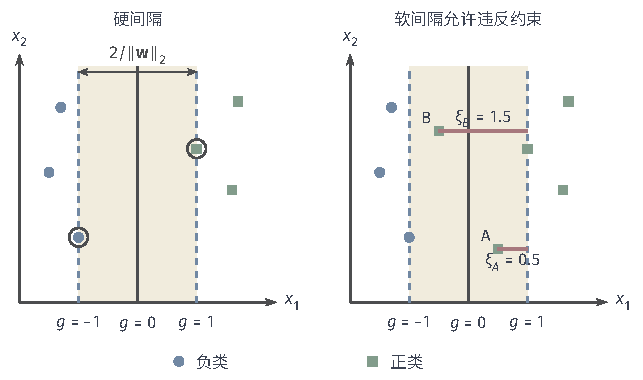
\includegraphics[width=108.850mm]{figures/04-classic-models/00-shared/tikz/classification-svm-margin/figure.pdf}
  \caption{硬间隔与软间隔的教学示意，坐标无量纲。蓝圆为负类，赭方为正类；两个面板都给定$\bm{w}=(1,0)^{\top}$、$b=-2$，黑色实线为决策边界$g=0$，蓝色虚线为间隔边界$g=\pm1$。单侧规范间隔为$1/\lVert\bm{w}\rVert_2=1$，两虚线总宽为$2/\lVert\bm{w}\rVert_2=2$；左图圈出间隔上的样本。右图红色线段直接标出松弛量：A位于$x_1=2.5$，正确分类但在间隔内，$\xi_A=0.5$；B位于$x_1=1.5$，已被错分，$\xi_B=1.5$。右图仅说明给定分界面下的最小松弛量，并非优化后的SVM最优解。}
  \label{fig:classification-svm-margin}
\end{figure}

消去$\bm{\xi}$，式\eqref{eq:classification-svm-soft-primal}等价于
\begin{equation}
  \min_{\bm{w},b}\quad
    \frac12\lVert\bm{w}\rVert_2^2
    +\lambda_{\mathrm{s}}\sum_{i=1}^n
       \max\{0,1-y_i g(\bm{x}_i)\}.
  \label{eq:classification-svm-hinge-objective}
\end{equation}
其中$\ell(z)=\max\{0,1-z\}$是\term{合页损失}（hinge loss）：达到目标间隔以后不再奖励更大的得分，间隔不足时线性增加惩罚。错误一侧的损失继续线性增加而不截断，保持了凸性。它把“最大间隔加违规代价”与“平方范数正则化加经验损失”联系起来。

惩罚参数的数值还依赖损失是求和还是取平均。将式\eqref{eq:classification-svm-hinge-objective}除以$n\lambda_{\mathrm{s}}$，等价目标是平均合页损失加$\lVert\bm{w}\rVert_2^2/(2n\lambda_{\mathrm{s}})$。所以在不同样本量或不同软件约定之间比较超参数时，应先统一归一化方式。较大的$\lambda_{\mathrm{s}}$允许模型付出更大范数来降低训练损失，较小的值更重视范数控制；范数和损失的取舍是否适合任务，需要结合数据、表示与验证结果判断。

软间隔的乘子上界来自松弛变量的最优性条件。分别为$1-\xi_i-y_i g(\bm{x}_i)\le0$与$-\xi_i\le0$引入$\alpha_i,\mu_i\ge0$，拉格朗日函数为
\[
  \begin{aligned}
    L={}&\frac12\lVert\bm{w}\rVert_2^2
       +\lambda_{\mathrm{s}}\sum_i\xi_i\\
      &+\sum_i\alpha_i
        \bigl[1-\xi_i-y_i(\bm{w}^{\top}\bm{x}_i+b)\bigr]
       -\sum_i\mu_i\xi_i.
  \end{aligned}
\]
关于$\bm{w},b$的驻点条件仍是式\eqref{eq:classification-svm-stationarity}，关于每个$\xi_i$则要求$\lambda_{\mathrm{s}}-\alpha_i-\mu_i=0$。结合$\mu_i\ge0$，得到$0\le\alpha_i\le\lambda_{\mathrm{s}}$。取$\bm{w}=\bm{0}$、$b=0$和所有$\xi_i>1$可以严格满足两组不等式，因此不论数据是否可分，\term{Slater条件}都成立。消去原始变量后有
\begin{equation}
  \begin{aligned}
    \max_{\bm{\alpha}}\quad&
      \sum_{i=1}^n\alpha_i
       -\frac12\sum_{i,j=1}^n
         \alpha_i\alpha_j y_i y_j
         \bm{x}_i^{\top}\bm{x}_j\\
    \text{s.t.}\quad&
      \sum_{i=1}^n\alpha_i y_i=0,\\
    &0\le\alpha_i\le\lambda_{\mathrm{s}},
      \qquad i=1,\ldots,n.
  \end{aligned}
  \label{eq:classification-svm-soft-dual}
\end{equation}
对偶可行域非空且紧，目标连续，所以对偶最优值可以取得。原始形式同样有最优解；两类非空时，限制目标的水平集可控制$\bm{w}$与$\bm{\xi}$，再由两类约束控制$b$。

软间隔的互补松弛关系多了一组：
\begin{equation}
  \begin{aligned}
    &\alpha_i^{\ast}(m_i^{\ast}-1+\xi_i^{\ast})=0,\\
    &(\lambda_{\mathrm{s}}-\alpha_i^{\ast})\xi_i^{\ast}=0,\\
    &m_i^{\ast}\ge1-\xi_i^{\ast},\qquad \xi_i^{\ast}\ge0.
  \end{aligned}
  \label{eq:classification-svm-soft-kkt}
\end{equation}
联合原始与对偶可行性，可以逐项读出
\begin{equation}
  \begin{aligned}
    \alpha_i^{\ast}=0
      &\ \Longrightarrow\
        \xi_i^{\ast}=0,\quad m_i^{\ast}\ge1,\\
    0<\alpha_i^{\ast}<\lambda_{\mathrm{s}}
      &\ \Longrightarrow\
        \xi_i^{\ast}=0,\quad m_i^{\ast}=1,\\
    \alpha_i^{\ast}=\lambda_{\mathrm{s}}
      &\ \Longrightarrow\
        m_i^{\ast}=1-\xi_i^{\ast}\le1.
  \end{aligned}
  \label{eq:classification-svm-soft-cases}
\end{equation}
边界上的样本可以出现在三种乘子状态中：$\alpha_i^{\ast}=0$允许$m_i^{\ast}=1$，$\alpha_i^{\ast}=\lambda_{\mathrm{s}}$也允许$\xi_i^{\ast}=0$且$m_i^{\ast}=1$。反过来，$m_i^{\ast}>1$必有$\alpha_i^{\ast}=0$，$m_i^{\ast}<1$必有$\alpha_i^{\ast}=\lambda_{\mathrm{s}}$，而$m_i^{\ast}=1$时乘子可以是盒约束中的任意值，只要整体KKT系统成立。达到上界的乘子因此可能对应边界点、间隔内的正确样本或错分样本，需要结合$m_i^{\ast}$才能区分。

范数项依然只对$\bm{w}$严格凸，足以保证最优权重唯一，却不能保证偏置唯一。一个简单反例是两个输入都为零，标签分别为$+1$与$-1$。此时$\bm{w}^{\ast}=\bm{0}$，任意$b\in[-1,1]$都使总合页损失为$2$，因此都最优。该情形也说明，软间隔可能得到常值得分；只有$\bm{w}\ne\bm{0}$时，才可以继续用$1/\lVert\bm{w}\rVert_2$解释规范间隔的几何宽度。

若存在$0<\alpha_k^{\ast}<\lambda_{\mathrm{s}}$的\term{自由支持向量}（free support vector），它既参与决策又未碰到乘子上界，可用$m_k^{\ast}=1$恢复偏置。若没有这种样本，就应使用KKT给出的偏置区间。令$h_i=\sum_j\alpha_j^{\ast}y_j\bm{K}_{j,i}$，则$\alpha_i^{\ast}=0$要求$y_i(h_i+b)\ge1$，$\alpha_i^{\ast}=\lambda_{\mathrm{s}}$要求$y_i(h_i+b)\le1$。正标签的前一条件与负标签的后一条件给出下界，另两种组合给出上界；从两组界的交集中选择一个$b$，才是完整的恢复规则。该区间不一定收缩为单点。

SMO的一元目标与误差公式不变，但可行区间必须同时保证两个乘子都位于盒子内。令$s=y_i y_j$，新的$\alpha_j$区间为
\begin{equation}
  \begin{aligned}
    s=+1:\quad
    L&=\max\{0,\alpha_i^{(t)}+\alpha_j^{(t)}
                    -\lambda_{\mathrm{s}}\},\\
    H&=\min\{\lambda_{\mathrm{s}},
                    \alpha_i^{(t)}+\alpha_j^{(t)}\};\\
    s=-1:\quad
    L&=\max\{0,\alpha_j^{(t)}-\alpha_i^{(t)}\},\\
    H&=\min\{\lambda_{\mathrm{s}},
           \lambda_{\mathrm{s}}+\alpha_j^{(t)}-\alpha_i^{(t)}\}.
  \end{aligned}
  \label{eq:classification-svm-smo-soft-interval}
\end{equation}
这是由盒约束与等式约束共同截出的区间，通常小于$[0,\lambda_{\mathrm{s}}]$。使用式\eqref{eq:classification-svm-smo-update}剪裁并回代即可；当$\eta=0$时，这里的区间总是有限，可以直接比较端点目标。偏置仍按式\eqref{eq:classification-svm-smo-bias}计算，但优先使用更新后满足$0<\alpha_i<\lambda_{\mathrm{s}}$或$0<\alpha_j<\lambda_{\mathrm{s}}$的样本；二者都不自由时，可暂取两个候选偏置的平均，停止时再按全体KKT条件核验。

在可分数据上，足够大的有限惩罚就能使软间隔与硬间隔精确对应。取任意硬间隔最优乘子$\bm{\alpha}^{\mathrm{h}}$，若$\lambda_{\mathrm{s}}>\max_i\alpha_i^{\mathrm{h}}$，则硬间隔原始解连同$\bm{\xi}=\bm{0}$、$\bm{\alpha}^{\mathrm{h}}$和$\mu_i=\lambda_{\mathrm{s}}-\alpha_i^{\mathrm{h}}>0$满足软间隔KKT。由强对偶它也是软间隔最优解，而且正的$\mu_i$迫使所有最优松弛量为零。若数据不可分，则无论把惩罚增大到多少，都不能恢复一个本来就不存在的硬间隔可行解。惩罚参数在训练集内部选择。

\subsubsection{支持非线性可分：核方法}
\label{sec:classification-svm-kernels}

原坐标中的仿射得分只能给出直线或超平面边界。例如第\ref{sec:classic-overview-kernel-trick}节的圆内、圆外分类，需要曲线边界；调整原坐标中的线性系数，并不能让边界变成这条圆。核化改为在特征空间中学习线性得分，让原输入空间中的边界可以是非线性的。

SVM的对偶已经只含训练样本内积，所以可以用正定核$K$替换这些内积，在不显式构造高维坐标的情况下训练和预测。逐对求值得到的$\bm K_{ij}=K(\bm{x}_i,\bm{x}_j)$是由训练输入直接算出的Gram矩阵，属于数据导出量，本身不是待学参数；训练学的仍是对偶乘子$\alpha_i$。核技巧与合法性的理由见第\ref{sec:classic-overview-kernel-trick}节，常用核见第\ref{sec:classic-overview-common-kernels}节；这里将它们代入SVM的目标，推导相应的对偶与预测规则。

将$\bm{w}\in\mathbb{R}^d$换成$\bm{w}\in\mathcal{H}$，将平方范数换成$\lVert\bm{w}\rVert_{\mathcal{H}}^2$，硬间隔的内积推导便可在特征空间中进行。更具体地，把任意$\bm{w}$分解为训练特征张成空间内的部分与其正交部分，后者不改变任何训练得分，却只会增加范数。因此最优权重可以限制在有限个训练特征的张成空间中；驻点条件进一步给出$\bm{w}^{\ast}=\sum_i\alpha_i^{\ast}y_i\bm{\phi}(\bm{x}_i)$。若还允许样本违反单位间隔，并以$\lambda_{\mathrm{s}}>0$惩罚每单位违反量，对偶乘子便增加同一数值的上界；这一软间隔构造已在前面展开。把硬间隔与这种允许违反的版本合写，核化对偶为
\begin{equation}
  \begin{aligned}
    \max_{\bm{\alpha}}\quad&
      \sum_{i=1}^n\alpha_i
       -\frac12\sum_{i,j=1}^n
          \alpha_i\alpha_j y_i y_j
          K(\bm{x}_i,\bm{x}_j)\\
    \text{s.t.}\quad&
      \sum_{i=1}^n\alpha_i y_i=0,\\
    &0\le\alpha_i\le\lambda_{\mathrm{s}},
      \qquad i=1,\ldots,n.
  \end{aligned}
  \label{eq:classification-svm-kernel-dual}
\end{equation}
在映射后严格可分的硬间隔情形，去掉乘子上界即可。新输入的得分与预测为
\begin{equation}
  \begin{aligned}
    g^{\ast}(\bm{x})
      &=\sum_{i\in S}\alpha_i^{\ast}y_i
         K(\bm{x}_i,\bm{x})+b^{\ast},\\
    \hat y(\bm{x})&=\operatorname{sign}(g^{\ast}(\bm{x})).
  \end{aligned}
  \label{eq:classification-svm-kernel-prediction}
\end{equation}
边界在$\mathcal{H}$中仍然是线性的，在原输入空间中则可能是曲线或曲面。SMO也只需把$\bm{K}_{i,j}$换成$K(\bm{x}_i,\bm{x}_j)$；此时$\eta=\lVert\bm{\phi}(\bm{x}_i)-\bm{\phi}(\bm{x}_j)\rVert_{\mathcal{H}}^2\ge0$，前面的区间、零曲率处理与偏置更新都继续适用。

不同核能表达的关系并不相同。二次多项式核$K(\bm x,\bm z)=(1+\bm x^\top\bm z)^2$的特征包含$x_1x_2$，所以候选得分$x_1+x_2-2x_1x_2-1/2$能精确区分前面的四点异或关系：两个负类点得分为$-1/2$，两个正类点得分为$1/2$。对RBF核$K(\bm x,\bm z)=\exp[-\|\bm x-\bm z\|_2^2/(2\sigma^2)]$，其中$\sigma>0$，候选得分$K(\bm0,\bm x)-t$在$0<t<1$时形成半径$\sigma\sqrt{-2\log t}$的球形正类区域。这里使用了一个核基函数与偏置，直接展示了直线表示缺少的半径关系。

这些例子只证明相应目标在候选得分族中，不保证训练必然找到它们。固定$p$次多项式核在一维仍只产生至多$p$次的多项式得分，非零得分至多有$p$个实根，因而不能表示任意多次交替的类别区间。范数、偏置和核尺度的限制又会约束可用得分及间隔；“使用核”本身不是对任意目标的逼近保证。

核合法性要求核矩阵在任意有限输入集上半正定；核尺度与特征预处理共同决定映射后能否分开。核技巧去掉了对显式特征维数的直接依赖，但没有去掉对样本量的依赖。构建完整Gram矩阵需要$O(n^2)$次核调用，之后还要执行优化迭代；两者合起来才是训练成本。若一次核计算耗时$t_K$，单次预测的主要核计算量是$O(|S|t_K)$，其中$|S|$为支持向量数量。训练存储与预测成本都由支持向量数决定；核化不同时解决标签噪声。无限维特征可以通过有限次内积运算使用，与“训练成本只由核计算决定”是两回事。

\subsubsection{调节间隔与违反比例：nu-SVM}
\label{sec:classification-svm-nu-extension}

软间隔惩罚系数衡量一单位间隔违反有多昂贵，却不能直接读成“允许多少训练样本违反间隔”。若希望调节参数与训练中的间隔错误比例、支持向量比例建立联系，可以考虑\term{$\nu$-SVM}（nu-support vector machine）。它把间隔阈值$\rho\geq0$也作为变量，在目标中用参数$\nu$奖励更大的阈值，同时惩罚平均松弛量：
\begin{equation}
  \begin{aligned}
    \min_{\bm{w},b,\rho,\bm{\xi}}\quad&
      \frac12\lVert\bm{w}\rVert_2^2-\nu\rho
      +\frac1n\sum_{i=1}^n\xi_i\\
    \text{满足}\quad&
      y_i(\bm{w}^{\top}\phi(\bm{x}_i)+b)\geq\rho-\xi_i,\\
    &\xi_i\geq0,\qquad \rho\geq0.
  \end{aligned}
  \label{eq:classification-nu-svm}
\end{equation}
消去原始变量后，可学习的仍是训练样本的非负系数，但对偶变为
\[
  \begin{aligned}
    \max_{\bm\alpha}\quad&-\frac12\sum_{i,j}\alpha_i\alpha_jy_iy_jK(\bm x_i,\bm x_j),\\
    \text{满足}\quad&0\leq\alpha_i\leq1/n,\quad
       \sum_i\alpha_i y_i=0,\quad\sum_i\alpha_i\geq\nu.
  \end{aligned}
\]
最后一个不等式来自原始问题中的$\rho\geq0$。固定核后可用凸二次规划求系数，再由原始约束和互补松弛恢复偏置及间隔阈值，预测仍对核展开得分取符号。这个目标与软间隔相似，却不是只把惩罚参数换一个名字。

使用时还需结合类别数量检查参数范围：两类训练样本数为$n_+$、$n_-$时，应限制$0<\nu\leq2\min(n_+,n_-)/n$。以下讨论达到精确最优、且最优间隔阈值$\rho^\ast>0$的非退化情形。记最优得分为$g^\ast$，满足$y_i g^\ast(\bm{x}_i)<\rho^\ast$的训练样本称为间隔违反样本；其中也包括已经分类正确、但尚未达到目标间隔的样本。此时，$\nu$是间隔违反样本比例的上界，也是非零对偶系数所对应支持向量比例的下界\scite{scholkopf2000nu}。

这两个方向可以从KKT条件读出。为间隔约束引入乘子$\alpha_i\geq0$。关于松弛变量的驻点条件给出$\alpha_i\leq1/n$；关于$\rho$的驻点条件与$\rho^\ast>0$的互补松弛关系给出
\[
  0\leq\alpha_i^\ast\leq\frac1n,
  \qquad \sum_{i=1}^{n}\alpha_i^\ast=\nu.
\]
这里仍有偏置的驻点条件$\sum_i\alpha_i^\ast y_i=0$，所以正、负两类的乘子总量相同，均为$\nu/2$。每项乘子至多为$1/n$，正类总量因而不超过$n_+/n$，负类总量不超过$n_-/n$。将这两项上界与$\nu/2$比较，就得到前面要求的$\nu\leq2\min(n_+,n_-)/n$；少数类的样本数量限制了两类能够共同承担的乘子总量。这也说明，上述类别数量条件与后面的比例解释都应结合当前模型及最优阈值条件检查。

令$E_\nu=\{i:y_i g^\ast(\bm{x}_i)<\rho^\ast\}$、$S_\nu=\{i:\alpha_i^\ast>0\}$。间隔违反样本的最优松弛量为正，因而乘子必须达到上界$1/n$；另一方面，要把每项至多$1/n$的非负乘子累加到$\nu$，至少需要$n\nu$个非零项。于是
\begin{equation}
  \frac{|E_\nu|}{n}\leq\nu\leq\frac{|S_\nu|}{n}.
  \label{eq:classification-nu-svm-proportions}
\end{equation}
例如，$n=100$、$\nu=0.2$且上述条件满足时，间隔违反样本至多有20个，支持向量至少有20个；这既不表示恰有20个错分样本，也不是对测试错误率的保证。若最优$\rho=0$，这里依据$\sum_i\alpha_i^\ast=\nu$得到的比例解释不能直接沿用。比例界、错分数和测试错误率三者必须区分；退化阈值下不能直接沿用解释。

固定核后，$\nu$-SVM与软间隔SVM使用同一得分族。它改变间隔的选取方式，不增加非线性特征，也仍需要检查核尺度、类别不平衡和独立验证误差。
